% Specify the type of document
\documentclass[12pt]{article}

% Load a number of useful packages
\usepackage{graphicx}
\usepackage{amsmath,amssymb,amsfonts,amsthm}
 \usepackage[margin=1.0in]{geometry}
\usepackage[colorlinks=true]{hyperref}
\usepackage{cite}
\usepackage[final]{pdfpages}
\usepackage[caption=false,font=footnotesize]{subfig}

\usepackage{listings}
\usepackage{color} %red, green, blue, yellow, cyan, magenta, black, white

\usepackage{setspace}
\doublespacing

\newcommand\scalemath[2]{\scalebox{#1}{\mbox{\ensuremath{\displaystyle #2}}}}


% Say where pictures (if any) will be placed
\graphicspath{{./pictures/}}

% Define title, author, and date
\title{OUFTI 1\\
  \large Attitude Determination and Control System}
\author{Emilio R. Gordon}
\date{March 13, 2018}


% Start of document
\begin{document}
% Put the title, author, and date at top of first page
\maketitle
{\singlespacing
\tableofcontents}
\newpage
%%%%%%%%%%%%%%%%%%%%%%%%%%%
%%%%%%%%%%%%                                    Section
%%%%%%%%%%%%%%%%%%%%%%%%%%%
\section{Introduction }
In 2016, the University of Leige developed the first nano-satellites ever made in Belgium: OUFTI-1. The satellite is led by students supported by professors much like our University's SatDev program. OUFTI-1 is a 1U cubesat and is the first satellite equipped with the amateur radio digital-communication protocol: D-STAR technology. OUFTI-1 is equipped with other experiments such as an innovative electrical power system and high-performance solar cells.\cite{eoPortal}\cite{SpaceFlight101}
%\newline \newline
%Due to its mission, OUFTI-1 is not required to point in one specific direction and the Attitude Determination and Control System (ADCS) subsystem relies on Passive Magnetic Attitude Stabilization (PMAS).
%\subsection{Attitude Determination and Control System Overview}
%Attitude referes to the orientation of a body-fixed coordinate frame with respect to an external inertial frame. The Attitude Determination and Control System is made of two parts: attitude determination and attitude control.
%\newline \newline
%Attitude determination is the process of measuring and determining a spacecrafts orientation. In the case of OUFTI-1, an accurate attitude determination was not necessary for mission success.
%\newline \newline
%Attitude control refers to the process of orienting the spacecraft to a given direction. The requirements for pointing accuracy, stability, and maneuverability, as well as other mission requirements such as cost, weight, reliability, orbital motion and lifetime were the key parameters that drove the decision on what technique for control was used. 
%%%%%%%%%%%%%%%%%%%%%%%%%%%
%%%%%%%%%%%%                                    Section
%%%%%%%%%%%%%%%%%%%%%%%%%%%
\section{Attitude Determination of OUFTI-1}
The goal of the attitude determination of OUFTI-1 was to get an estimation of the in-orbit rotational speed to provide comparisons to the simulations performed\cite{adcs} . Though there are many sensors on market that can determine attitude, none were used aboard OUFTI-1. It was advantageous to use the existing solar panels as analogue sun sensors. The accuracy, though rough, out-weighed the cost of adding any sensors on-board. 
\newline \newline
Recall that OUFTI-1 is equipped with high-performance solar cells. With information on the power received on each side of the satellite, the position of the sun with respect to the satellite can be determined. As a result, the solar panels act as a two-axis sun sensor with a precision of a couple degrees. 
\newline \newline
This approach for attitude determination lacked the ability to retrieve any information on the angular velocity of the satellite around the sun vector. As a result, information retrieved on the angular velocity was perpendicular to the sun vector.\cite{adcs} 
%%%%%%%%%%%%%%%%%%%%%%%%%%%
%%%%%%%%%%%%                                    Section
%%%%%%%%%%%%%%%%%%%%%%%%%%%
\section{Passive Attitude Control of OUFTI-1}
OUFTI-1's mission did not require any high-precision orientation or specific maneuvers. As a result, passive attitude controls were the best solution of attitude control since it is cheap, simple, light-weight and consumes no power. In addition, passive attitude control does not require information regarding attitude inorder to work properly.
\newline \newline
There are two main passive control methods for satellites. One approach uses a gravity gradient leading to two stable states with the minor axis (axis with smallest moment of inertia) pointing towards the Earth. The other passive system orients the satellite along the Earth's magnetic field using an onboard magnet. In the case of OUFTI-1, the use of gravity gradient would have complicated the design. As such, OUFTI-1 utilizes passive magnetic attitude stabilization (PMAS).\cite{adcs} 
\newline \newline
Unless some means of damping is provided, the spacecraft will oscillate which is undesirable. This drawback was overcome by adding a damper that converts rotational energy into heat. Hysteresis damping is a desirable damping method for Low Earth Orbit spacecrafts used on OUFTI-1.\cite{adcs} 
%%%%%%%%%%%%%%%%%%%%%%%%%%%
%%%%%%%%%%%%                             SubSection
%%%%%%%%%%%%%%%%%%%%%%%%%%%
\subsubsection{Requirements}
To summarize, the goal for OUFTI-1 ADCS was to align the body-frame in the direction of the magnetic field using permanent magnets and to stabilize oscillations via hysteresis damping. A strong mathematical simulation including: environmental factors; magnetic and hysteresis phenomena; and satellite dynamics had to of been created in order to approach the attitude control.\cite{adcs}. The requirements set for the attitude control of OUFTI-1:\cite{adcs} 
\begin{itemize}
\item The tolerable stabilization time must be no more than one month.
\item After stabilization, the deviation from Earth's magnetic field must not exceed 15$^{\circ}$.
\end{itemize}
%%%%%%%%%%%%%%%%%%%%%%%%%%%
%%%%%%%%%%%%                       SubSubSection
%%%%%%%%%%%%%%%%%%%%%%%%%%%
\subsubsection{Magnet Material Selection}
Magnet selection for OUFTI-1 was between AlNiCo and Neodymium Iron bore (NdFeB). Material selection relied on two magnetic properties, remanence and coercivity. Remanence measures the strength of the magnetic field created by the magnet while Coercivity is the materials resistance to becoming demagnetized. The two materials shared very similar remanence however, AlNiCo-5 has a much lower coercivity. AlNiCo-5 was ultimately chosen due to pricing and flight experience. Despite it's low coercivity, these effects were able to be ignored with added precautions placed to handling and storage.
%%%%%%%%%%%%%%%%%%%%%%%%%%%
%%%%%%%%%%%%                       SubSubSection
%%%%%%%%%%%%%%%%%%%%%%%%%%%
\subsubsection{Hysteresis Damping}
Hysteresis is a lag which occurs between the application of a field/force and its subsequent effect. In magnetic hysteresis, it is the lag between a varying magnetic field, "H-field", and the subsequent magnetic induction. The energy loss per cycle is proportional to the area of the hysteresis loop. As the satellite rotates in low earth orbit, the hysteresis rods experience the effects of earth magnetic field which varies along its length. The magnetization of the rod then undergoes a hysteresis cycle and consequently is dissipated as heat, thus providing a damping term.
\newline \newline
The hysteresis bars were ultimately chosen to be made out of Permenorm 5000 H2, a soft magnetic nickel and iron alloy. Basic calculations were computed amongst different materials to find the energy loss per cycle with Permenorm 5000 H2 experiencing $7.75 \frac{J}{m^3}$ in one cycle. In addition, the material has space-flight experience making it more reliable than other material choices. \cite{adcs}
\newline \newline
Extensive simulations were computed to determine the hysteresis material alignment on the craft and its effect on damping efficiency and final stabilization. The damping efficiency is determined by the hysteresis rods volume. Since the length of the rods was limited to the size of a cube-sat, multiple parallel bars were be used. This maintained rod efficiency while also increasing the volume. The parallel rods however, were kept distant from each other in order to avoid mutual demagnetization.\cite{adcs}
%%%%%%%%%%%%%%%%%%%%%%%%%%%
%%%%%%%%%%%%                       SubSubSection
%%%%%%%%%%%%%%%%%%%%%%%%%%%
\subsubsection{Passive Magnetic Attitude Stabilization (PMAS) Design}
A major concern for the design of PMAS was the magnet's interaction with the hysteric bars as this limits the magnetic moment of the magnet. This concern forced a design with sufficient distances between the magnet and the hysteric materials which was particularly tricky on a cubesat. In addition, if a component of the magnet's field is directed along the rod, then there is a displacement of the working point observed in the hysteresis cycle. As a result, the ideal arrangement for the rods was to be as close as possible to the plane that is perpendicular to the permanent magnet axis\cite{adcs}. Any displacement from this plane would've lead to a component of the magnetic field directed along the hysteresis rod, thereby affecting the damping efficiency.
\newline \newline
For the official design of OUFTI-1, the exact PMAS configuration calls for the permanent magnet at the center of the edge between the face -X and +Z. For the location of the hysteresis rods, 4 bars were used lining the (-Y, +Z ) and (+Y,+Z) face as shown in the figure below. The results of this configuration allowed for a decrease angular rate of $8\times10^{-8} [\frac{rad}{sec^2}]$ which suggests a stabilization time of about 15 days.\cite{adcs}
\begin{center}
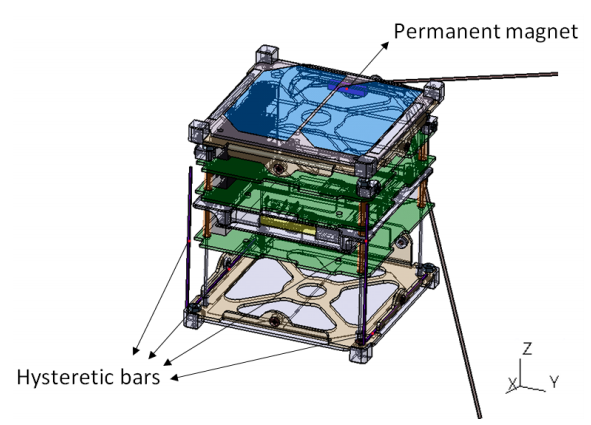
\includegraphics[scale=0.8]{1.png}
\end{center}
%%%%%%%%%%%%%%%%%%%%%%%%%%%
%%%%%%%%%%%%                             References
%%%%%%%%%%%%%%%%%%%%%%%%%%%
\begin{thebibliography}{9}
\bibitem{eoPortal} 
eoPortal Directory,
\textit{OUFTI-1 (Orbital Utility For Telecommunication Innovation)},
\\\texttt{https://earth.esa.int/web/eoportal/satellite-missions/o/oufti-1}

\bibitem{SpaceFlight101} 
Space Flight 101,
\textit{OUFTI-1},
\\\texttt{http://spaceflight101.com/spacecraft/oufti-1/}

\bibitem{adcs} 
Vincent Francois-Lavet, University of Li�ge, 2009-2010,
\textit{Study of passive and active attitude control systems for the OUFTI nanosatellites},
\\\texttt{http://vincent.francois-l.be/OUFTI\_ADCS\_2010\_05\_31.pdf}

\end{thebibliography}
\end{document}